HestiaPi's case comes in 2 parts. The backplate that goes to the wall and
should not be visible and the front cover. The backplate should have 4 small
holes, 3 larger holes and an opening for the wires coming from the wall.

If you bought HestiaPi, all internal screws are replaced with plastic rivets.
Otherwise you would need:

\begin{itemize}
\item 4 x 2.5Mx25mm hex screws
\item 4 x 2.5M hex nuts
\end{itemize}

For attaching to the wall you need:
\begin{itemize}
\item 4 x 3.5Mx40mm non-countersunk screws
\end{itemize}

Place the hex screws through the 4 small holes entering from the side facing
the wall. Secure them in the hex slot and make sure they are sit flush. Remove
the LCD from the PCB and insert the PCB alone guiding the 4 screws through the
4 corner holes of the Pi and secure with the nuts. Avoid using a large tool.
You can simply tighten them by hand. Don't overtighten.

With the remaining 3 larger holes mark your wall and drill according to the
location of the wires. The opening of the backplate should match the location
of the wires. Secure the backplate and PCB with the 3 larger screws.

Complete wiring according to your model instructions (for US see \ref{fig:us};
for EU see \ref{fig:eu})

\begin{figure}
  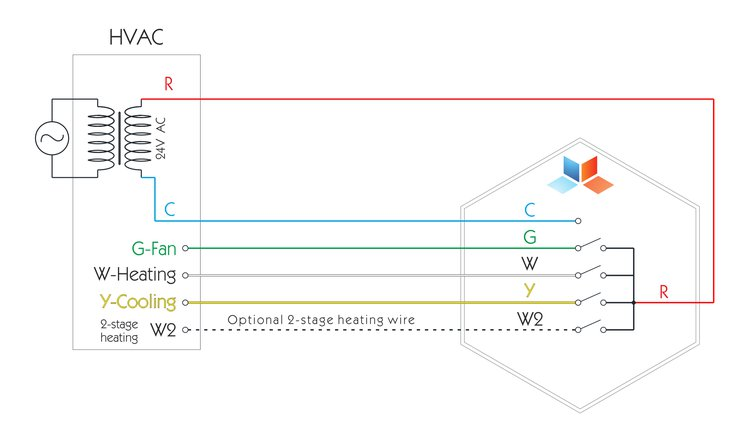
\includegraphics[width=5.0in]{img/US-hvac-wiring-diagram.jpg}
  \caption{US Wiring Diagram}
  \label{fig:us}
\end{figure}

\begin{figure}
  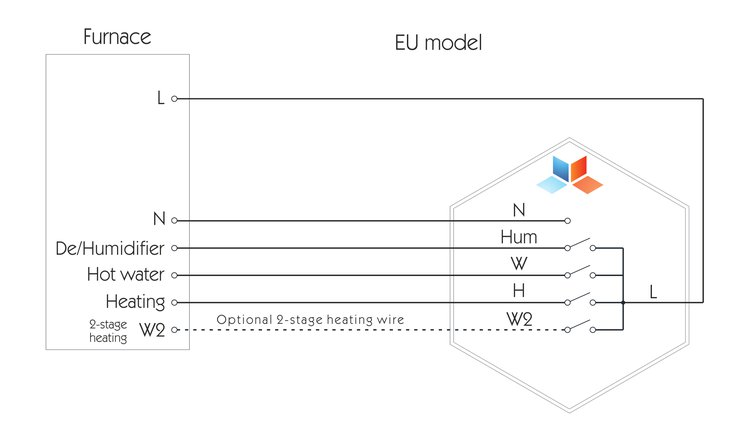
\includegraphics[width=5.0in]{img/eu-wiring-diagram.jpg}
  \caption{EU Wiring Diagram}
  \label{fig:eu}
\end{figure}

Remove any protective film from the LCD if present and lock the LCD on the
cover from the inside making sure the LCD's header is at the top.

Guide the 4 wires through the slit of bottom partition of the cover and secure
the sensor in it so that it is thermally protected from the rest of the
circuit.

If you installed the bottom screw it may block the cover to fully insert. Clip
off part of the sensor partition to allow enough clearance.

Hold the front cover aligned to the backplate and bring closer while you make
sure the pin header of the PCB is aligned to the header of the LCD. Push firmly
from the sides of the cover and not from the LCD till it locks in place. Make
sure no wires are caught in between as this may block the cover from locking in
place securely.
